\documentclass{article}
\usepackage{graphicx} % Required for inserting images
\usepackage{float}


\title{24.04.09 Bridge approach and BLS cost}
\author{Xun Zhang \quad \quad Bingsheng Zhang \\ 
Zhejiang University, CHN \\
22221024@zju.edu.cn \quad bingsheng@zju.edu.cn}

\date{April 09 2024}

\begin{document}

\maketitle

\section{Succinct labs Approach}

\subsection{Succinct 2022}
\begin{itemize}
    \item \textbf{Ethereum PoS Light Clients}. The Altair hard-fork to the Ethereum beacon chain introduced the \textbf{sync committee protocol} to allow for very compute-efficient light clients. The sync committee is a group of 512 validators assigned randomly from the full set of Beacon chain validators according to the RANDAO. The sync committee rotates every 256 epochs (roughly once every 27 hours). It's important the group of validators in the sync committee rotates periodically for security reasons.

    An honest validator chosen for sync committee participation is responsible for signing blocks. For each block that the sync committee signs, one member of the sync committee subset is responsible for producing an aggregate BLS signature and bitmap of the participating committee members, to produce a \textbf{SyncAggregate} container with this information, which gets gossiped at the p2p layer.

    There are 3 types of updates:
    \begin{itemize}
        \item \textbf{LightClientOptimisticUpdate} contains a block header that has not yet been finalized along with the corresponding SyncAggregate with the aggregate BLS signature and bitmap.
        \item \textbf{LightClientFinalityUpdate} contains an attested header that the sync committee has signed along with a finalized header that has been finalized according to the Casper FFG finality gadget. The update contains a merkle proof of the finalized header in the attested header.
        \item When the next sync committee is known (at least 1 epoch ahead of time) the light client receives a \textbf{LightClientUpdate}, which contains an attested header that the sync committee signs, along the next SyncCommittee and a merkle proof that the next sync committee is contained in the attested header.
    \end{itemize} 



    \item \textbf{Existing Problem}. Recall that the validator set of the sync committee rotates every 27 hours. On chain, we keep track of a commitment to the set of validators in the mapping \textbf{syncCommitteeRootByPeriod}. To update this mapping for the next period, we verify the merkle inclusion proof that the current validator set signs for the commitment for the next validator set.


    Unfortunately, the commitment the validators sign is an \textbf{SSZ commitment} (simple serialization, Eth PoS serialization format) that is quite SNARK unfriendly, as it uses the \textbf{SHA-256} hash function. It takes ~70 million constraints in a Groth16 circuit to compute the serialization of 512 validator BLS public keys to its corresponding SSZ commitment. 
    
    To address this, we use an additional SNARK to provably map an SSZ commitment to a SNARK-friendly \textbf{Poseidon} commitment. For each BLS signature verification, we pass in the poseidon commitment of the sync committee validators as public input to ensure that the BLS signature we are verifying is from the correct public keys. The commitment mapping SNARK must only be run every sync committee period (roughly once every 27 hours).


    \item \textbf{ZK-SNARK}. Thus there are two proof task: \textbf{Aggregated BLS Signature Verification} and \textbf{Sync Committee Commitment Mapping}.
    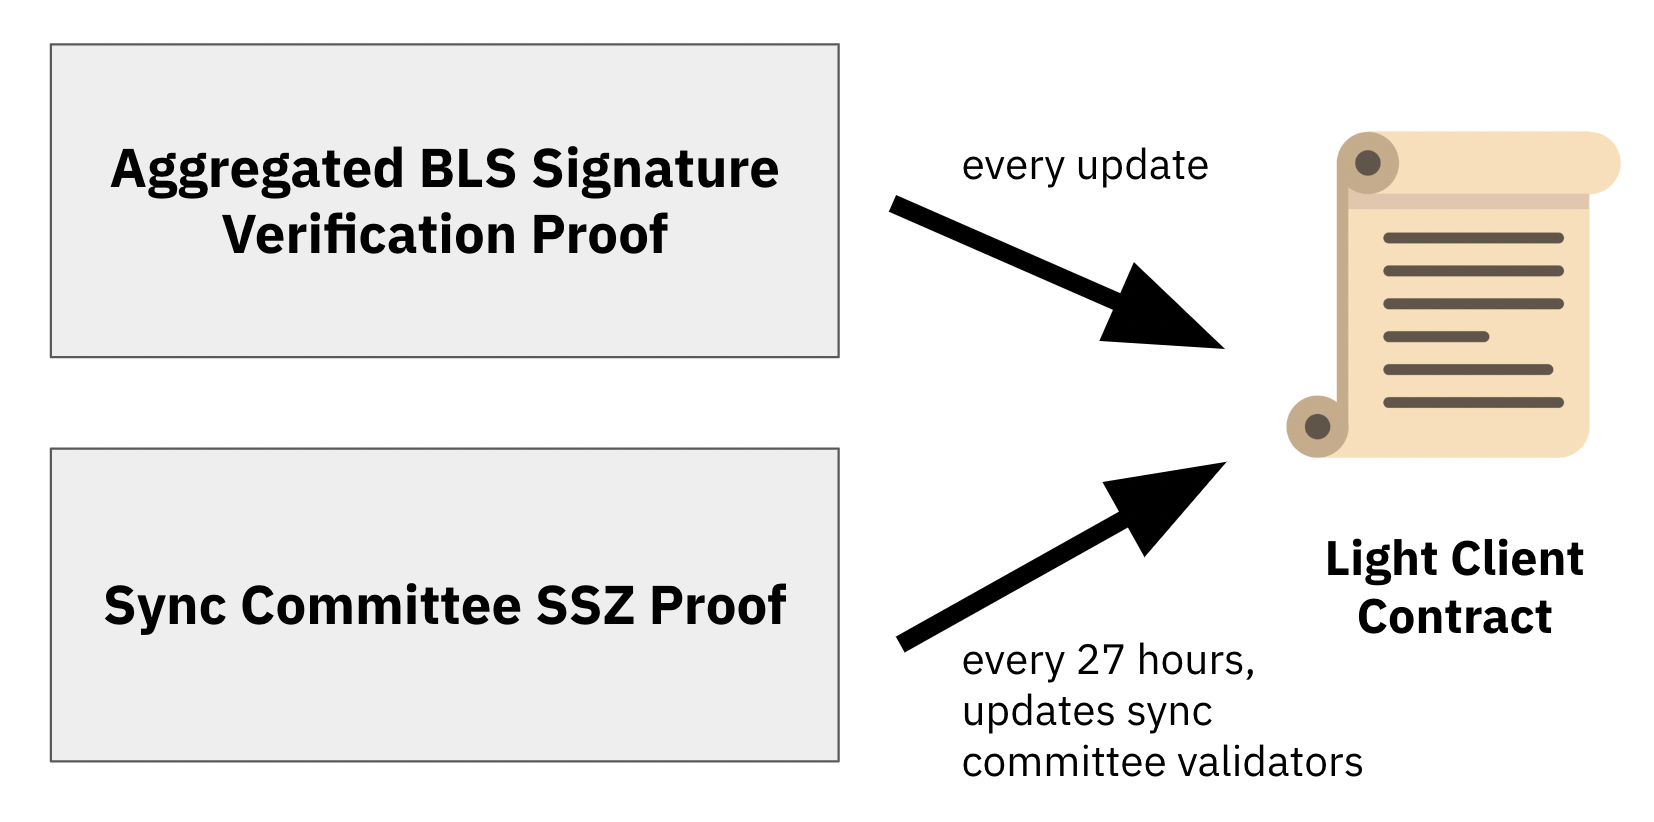
\includegraphics[width=1\linewidth]{Z0J8h33.png}

    (Succinct labs choose \textbf{Circom} and \textbf{Groth16} to generate zk-snarks)
 
    \begin{itemize}
        \item \textbf{Aggregated BLS Signature Verification}. To optimize the gas costs of the on-chain light client, we only store on-chain a SNARK-friendly commitment to the current set of public keys that govern the sync committee (as opposed to storing all 512 public keys in smart contract storage, which would be quite expensive). 

        The SNARK-friendly commitment is not normally available in the block headers, so we use the ZK-SNARK described below to map the SSZ commitment that is normally available in the block header to a more SNARK-friendly commitment that uses the \textbf{Poseidon} hash function.

        \item \textbf{Sync Committee Commitment Mapping}. This SNARK takes in a signed block header and maps the nextSyncCommitteeRoot field (the SSZ hash of the next validator set) to a SNARK-friendly \textbf{Poseidon} hash of the validator set. 

        We store this SNARK-friendly commitment on-chain and use it as an input to the BLS signature verifcation SNARK to ensure that the signature we are verifying is indeed from the sync committee validators. This circuit runs every 27 hours, for every sync committee rotation.
    \end{itemize}
\end{itemize}


\subsection{Succinct 2024}

Use SP1 to construct Zk bridge.

"\textit{We’re excited to announce Succinct Processor 1 (SP1): our first-generation \textbf{zero-knowledge virtual machine (zkVM)} that verifies the execution of arbitrary Rust (or any LLVM-compiled language) programs. SP1 targets an order of magnitude performance improvement vs. existing zkVMs—its alpha release is already up to 28x faster for certain programs and competitive with circuit-based approaches.}"


"\textit{SP1 achieves state-of-the-art performance on several real-world workloads inspired by common blockchain use-cases like bridging and verifying Merkle proofs. Our performance is a result of multiple design choices that utilize the latest proof system advances, including a cross-table lookup architecture, a customizable “precompile” system that can accelerate almost any performance bottleneck without much additional recursion overhead, and more. }"

~\\

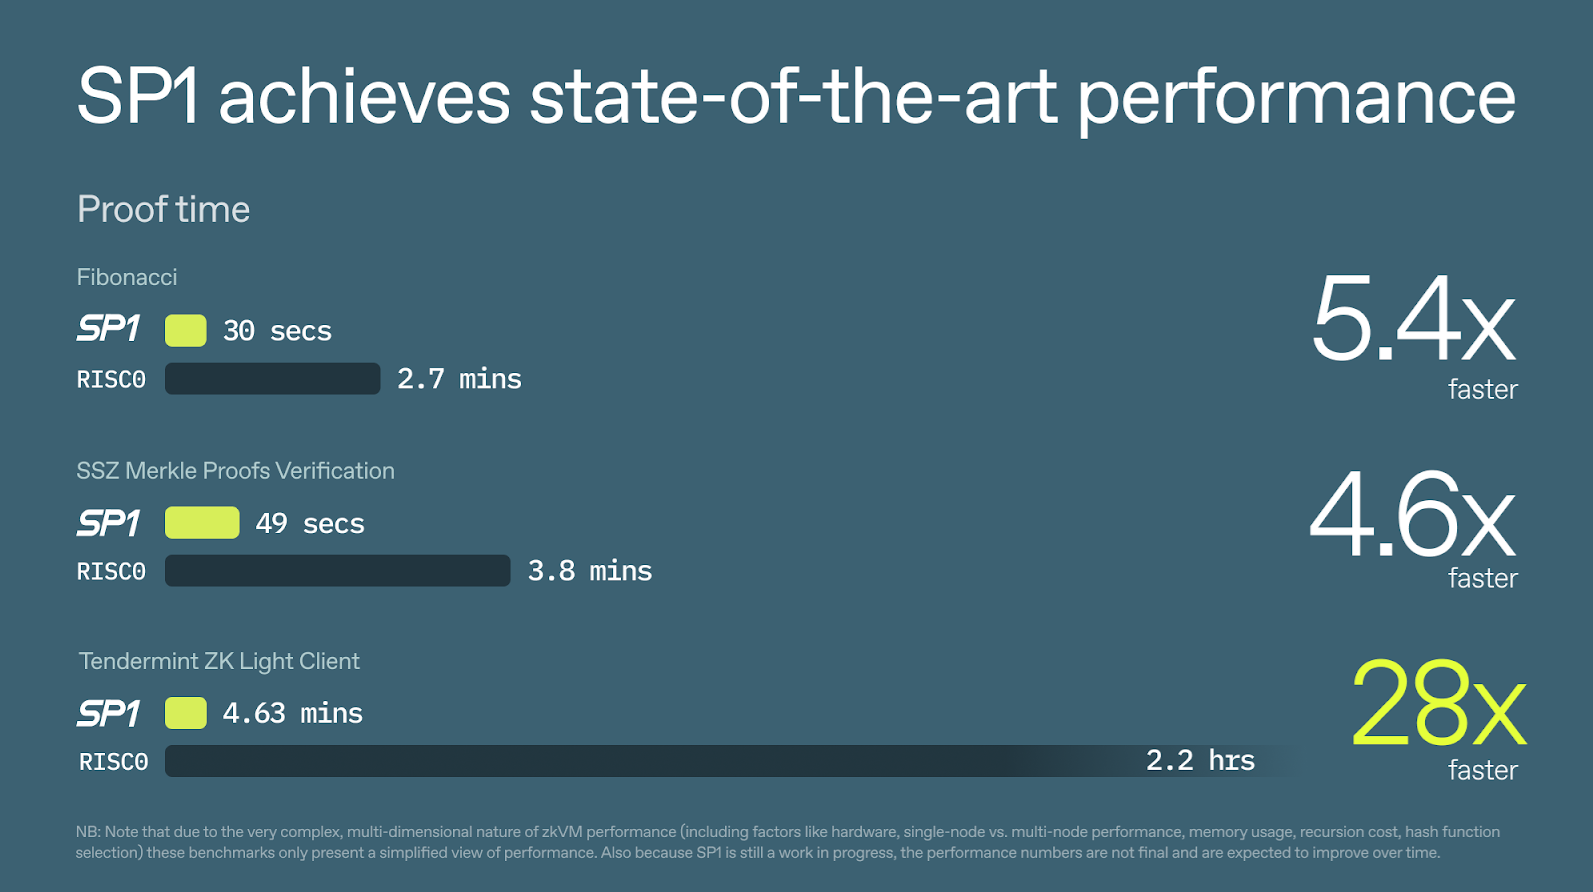
\includegraphics[width=1\linewidth]{SP1.png}



\section{ZKIBC Approach}

\subsection{ZKIBC 1.0}
We briefly introduce the ZKIBC 1.0 approache:

Electron labs have built a circom-based library that allows you to generate a zk-snark proof for a batch of Ed25519 signatures. 

Ed25519’s twisted Edwards curve uses a finite field that is larger than that used by the altbn128 curve (used by zk-snarks). Performing large finite field operations inside a smaller field is difficult because several basic operations such as modulo and multiplication can become very inefficient.

To solve this problem, Electron labs were able to find $2^{85}$ as a base over which to define our curve operations for twisted Edwards curve. Since the ed25519 prime p = $2^{255}$ - 19 is a close multiple of $2^{85}$, we were able to come up with efficient basic operators such as multiplication and modulo (under 25519 prime) for base $2^{85}$ numbers.

The proof parameters are following:
\begin{itemize}
    \item Proof generation time per signature ~ 9.6s (averaged out).
    \item Number of Signatures per batch/proof $\leq$ 100 (maximum value).
    \item Time to generate zk-proof for the batch = 16 mins for 100 signature batch.
\end{itemize}

Since the tendermint block production rate is ~ 7 sec and the proof generation time is 8 minutes, need multiple prover machines in parallel to keep up with the block production rate.

Number of parallel machines required = 8 mins *60 / 7 sec = 69 machines.



\subsection{ZKIBC 2.0}

The Solution of ZKIBC 2.0 is simple -- aggregate individual zk-proofs from multiple chains into a single "superproof". This enables the cost of proof verification to be amortised across many chains. The current state of the art ZK-tech already enables us to aggregate a large number of cosmos chains, with reasonable proving costs.

Assuming a proof verification gas cost of 250K, and N Cosmos chains being aggreagted, the cost per chain is 250K/N. For N =10, the cost per chain is 25,000, which is roughly the cost of an Eth transfer. As we add more and more chains into the network, the proof verification cost per chain continues to reduce and tends to zero, till the point the zk-hardware cost dominates.

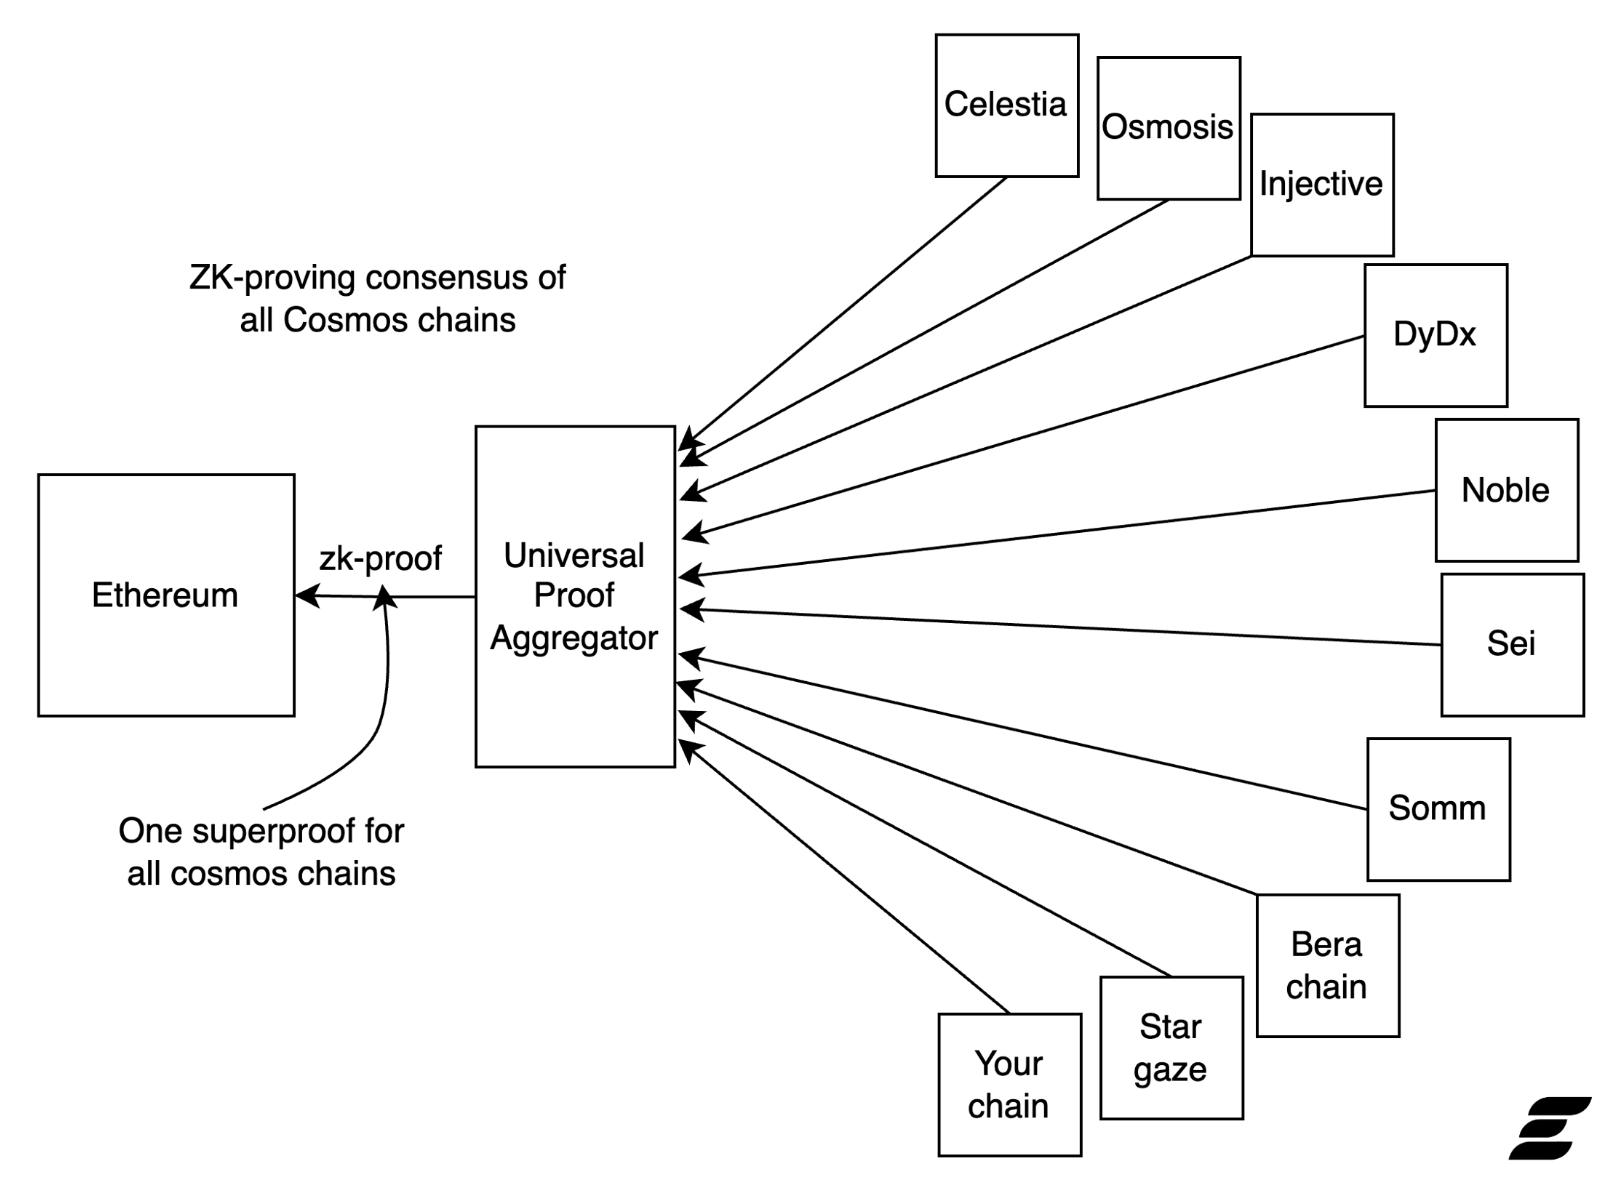
\includegraphics[width=1\linewidth]{ZKIBC2.png}

In ZK-IBC 1.0, we proved a single light header inside the circuit. This enabled us to reduce the information to be posted on-chain to a single hash string + the zk-proof itself.

With ZK-IBC 2.0, we are going one step beyond, rather than posting one hash string for each block of a chain, we create a merkle tree out of the individual hash strings from each chain, creating one superhash for all cosmos chains.

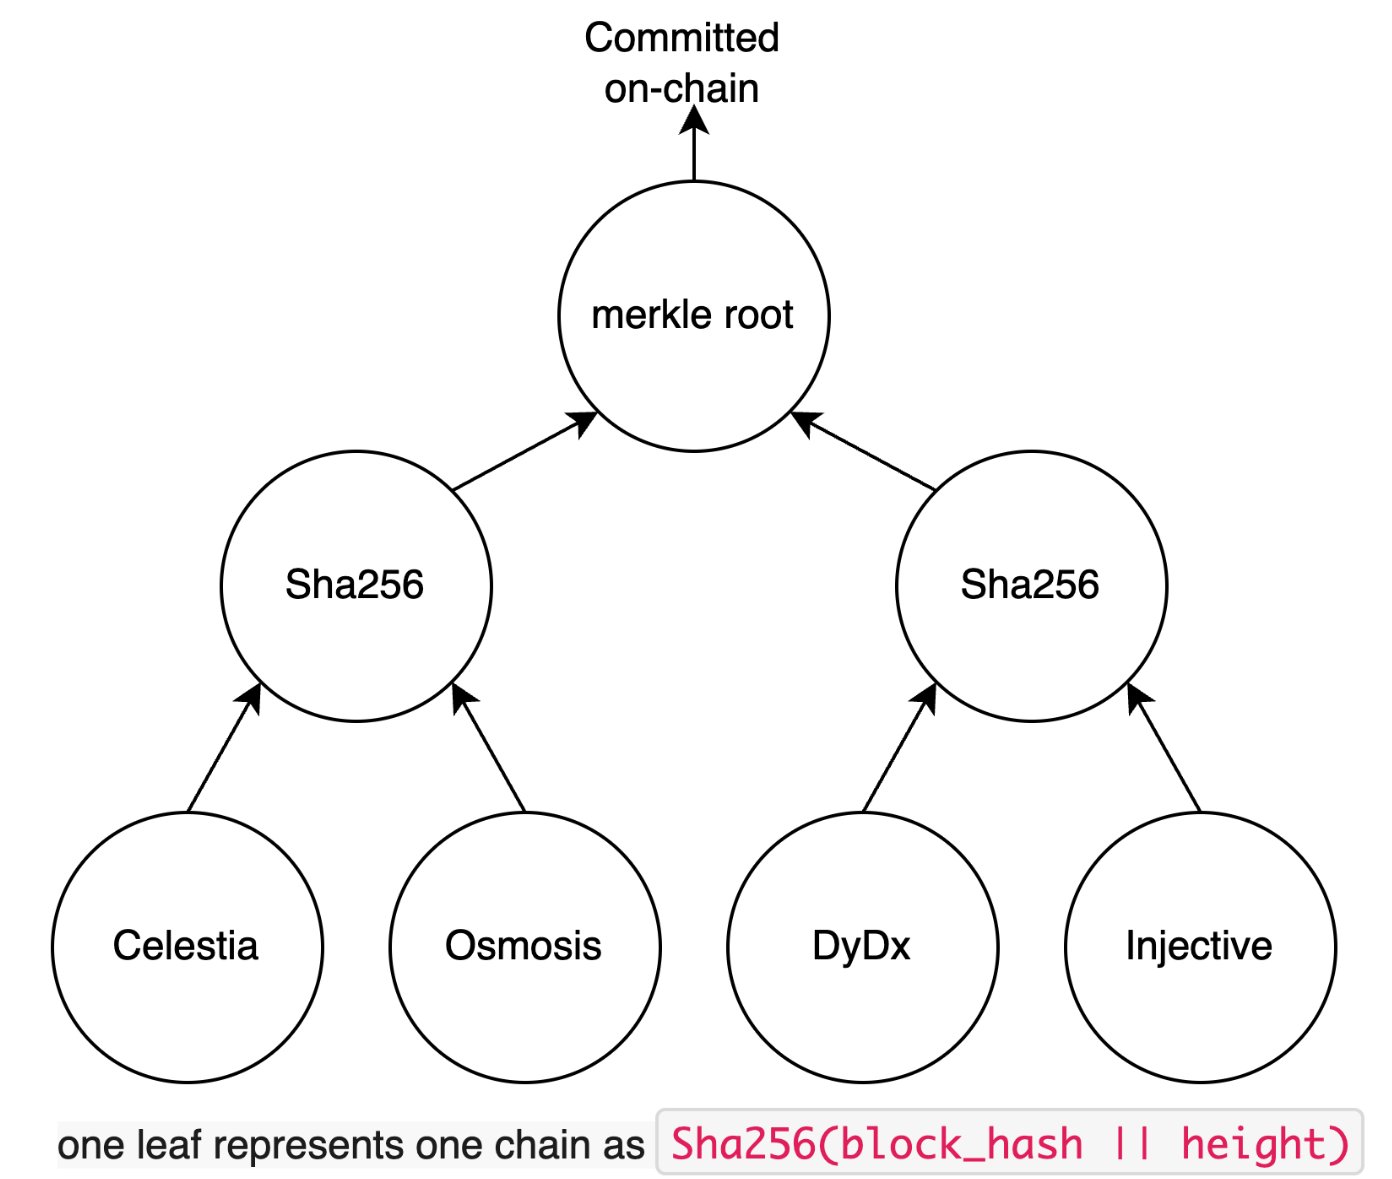
\includegraphics[width=1\linewidth]{ZKIBC_merkle.png}

~\\

\textbf{Prover infrastructure}. ZKIBC 2.0 has the following proof generation flow:
\begin{itemize}
    \item Generation of plonky2 proofs for individual chains. These machines run in parallel. Hence, when calculating Total Proving Time, we only need the maximum of the times taken by individual chains' machines.
    \item Aggregation of individual plonky2 proofs into a single aggregated plonky2 proof.
    \item Reduction of aggregate plonky2 proof to groth16 proof (the final superproof) to further reduce the cost of verifying the proof on-chain.
\end{itemize}


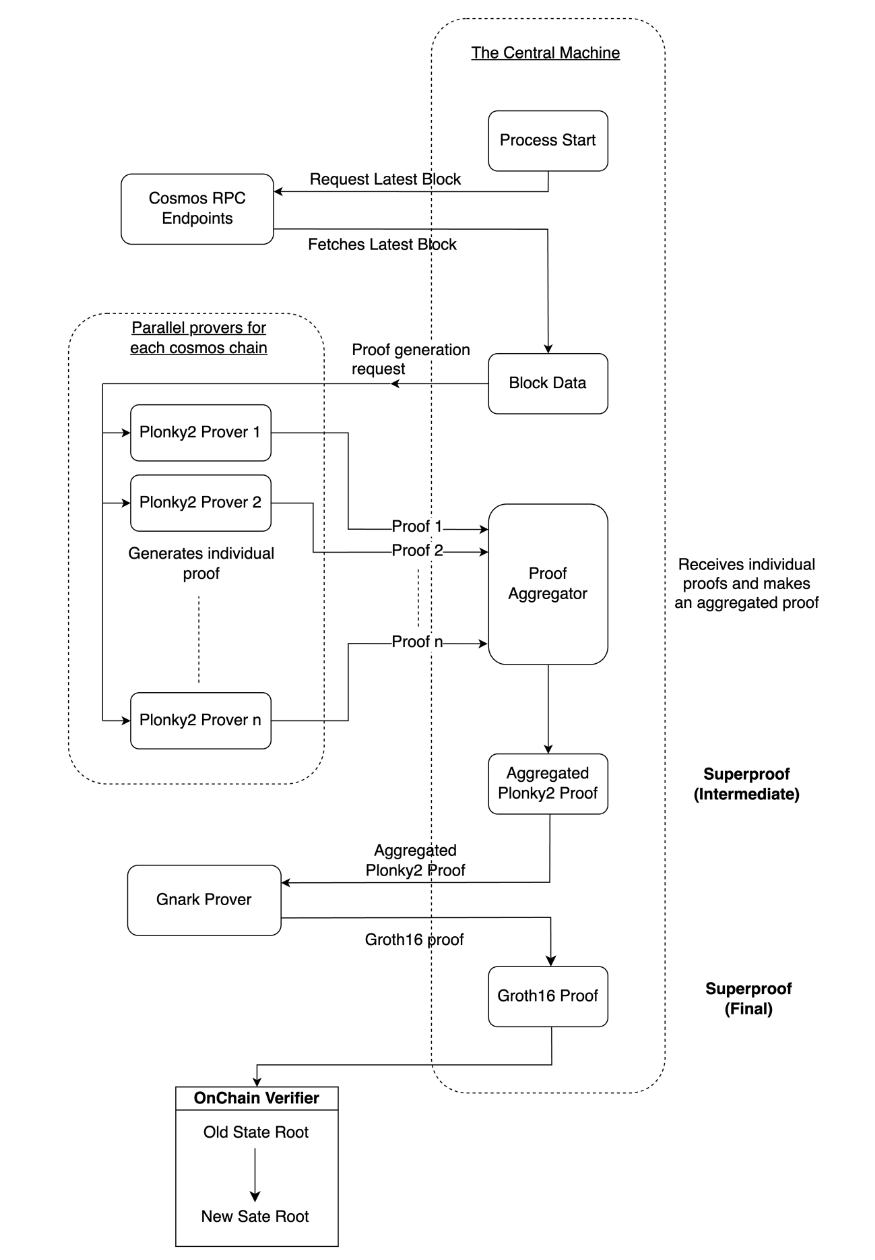
\includegraphics[width=1\linewidth]{ZKIBC_prover.png}




\section{BLS cost}

We also estimated the cost of various operations(mainly signature scheme) on the Cardano.

The aggregate BLS signature schemes have two versions. Single key version has the same key and different messages, with public key over G1. This
function returns a list of 10 messages \{'msg\_1', ..., 'msg\_10'\}, a public key 'pk', and an aggregate signature 'aggr\_sig'.

Multi key version has same message, with public key over G2. This function returns a message 'msg', ten public keys '\{pk\_1,...,pk\_10\}', and an aggregate signature 'aggr\_sig'.


\begin{table}[H]
    \centering
    \begin{tabular}{p{5cm}|p{2cm}|p{3cm}|p{3cm}} \hline
         Operation& Script size & CPU usage& memory usage  \\ \hline
         BLS Verification(G1)& 332  &    1,463,720,946   &  5754 \\ \hline
         BLS Verification(G2)& 380  &    1,342,066,427   &  5754 \\ \hline
         AggSig Verification(single key) &  777  &     3,336,910,422 &        71202   \\ \hline
         AggSig Verification(multi key) & 1704  &    3,676,891,887          &430586   \\ \hline
         Schnorr Verification(G1)  & 370   &     248,136,411   &          13796 \\ \hline
         Schnorr Verification(G2)  & 514    &    493,212,089    &         13964 \\ \hline
    \end{tabular}
    \caption{Cost of signature verification on BLS12-381}
    \label{tab:my_label}
\end{table}


\end{document}
